\documentclass{article}
\usepackage[utf8]{inputenc}
\usepackage[spanish]{babel}
\usepackage{listings}
\usepackage{graphicx}
\graphicspath{ {images/} }
\usepackage{cite}
\usepackage{amssymb, amsmath}

\begin{document}

\begin{titlepage}
    \begin{center}
        \vspace*{1cm}
            
        \Huge
        \textbf{Parcial 1: Informática II}
            
        \vspace{0.5cm}
        \LARGE
       Análisis y diseño.
          
            
        \vspace{5cm}
            
        \textbf{
        JOSE MIGUEL GOMEZ MONSALVE
        ERIKA LEÓN QUIROGA\newline
        DAVID AGUDELO OCHOA
        }
        
        
        
            
        \vfill
            
        \vspace{0.8cm}
       
        \Large


        \vfill
        Despartamento de Ingeniería Electrónica y Telecomunicaciones\\
        Universidad de Antioquia\\
        Medellín\\
        Febrero 2022
                 
    \end{center}
\end{titlepage}

\tableofcontents\newpage
\section{Introducción}
\noindent

\newpage

\section{Integrado 74HC595.} \label{Integrado}
El integrago 74HC595 hace parte de la familia de dispositivos SNx4HC59, la cual contienen un registro de desplazamiento de 8 bits de entrada en serie y salida en paralelo, el registro de almacenamiento tiene salidas de 3 estados paralelos. Se proporcionan relojes separados para el registro de desplazamiento y el de almacenamiento. El registro de desplazamiento tiene una entrada de anulación directa (SRCLR), una entrada en serie (SER) y salidas en serie para la conexión en cascada. Tienen una amplia corriente de funcionamiento de 2 V a 6 V, y las salidas de 3 estados de alta corriente pueden controlar hasta 15 cargas LSTTL. Los dispositivos tienen un bajo consumo consumo de 80-μA (máximo) ICC.
\subsection{Características del integrado.}\label{caracteristicas}
 \begin{itemize}
 
\item Entrada serial, salida paralela, o salida serial que permite la conexión en cascada de varios integrados.
\item Registro de desplazamiento de 8 bits que alimenta a un registro de almacenamiento.
\item Entradas de reloj separadas para el registro de desplazamiento y el de almacenamiento con activación por flanco de subida.

\end{itemize}

\begin{figure}[h]
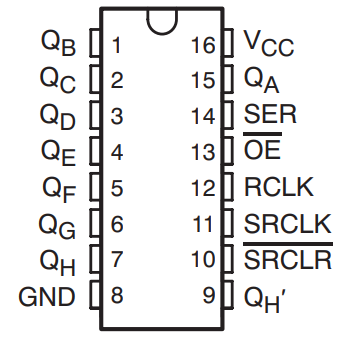
\includegraphics[scale=1]{esquematico.png}
\centering
\caption{Integrado 74HC595.}
\label{fig:int74HC959}
\end{figure}

\textbf{Configuración de pines.}
\newline
\begin{itemize}
\item Los pines de $Q_B$(pin 1) a $Q_H$(pin 7), añadiendo $Q_A$(pin 15) representan las salidas del integrado.
\item $V_C_C$(pin 16) es la alimentación y GND(pin 8) se conecta a tierra.
\item $Q_H_'$(pin 9) se utiliza para conectar otro integrado 74HC595 y generar un efecto de cascada.
\item El pin 14 o SER es el pin donde se envían los datos.
\item $\Bar{OE}$(pin 13) llamado Output Enable, habilita las salidas y se activa con un nivel bajo, por lo cual, para que siempre esté activo se conecta a GND.
\item El RCLK (pin 12) es el reloj del registro de almacenamiento y se utiliza para actualizar los datos a los pines de salida.
\item El SRCLK (pin 11) es el reloj que sincroniza la carga de datos.
\item El $\Bar{SRCLR}$ (pin 11) llamado Shift Register Clear, reestablece el registro de desplazamiento.


\end{itemize}

\subsection{Funcionamiento.}\label{integrado funcionamiento}
El objetivo principal es pasar el número dado de un formato serial a uno parelelo. Para explicar el funcionamiento del integrado tomaremos un número cualquiera de 8 bits, este número se irá guardando bit por bit en cada uno de los cuadros que se pueden ver en la Figura \ref{fig:func1}, también podemos ver en esta misma figura que la entrada de los datos es en serie (uno por uno), y la salida de ellos es en paralelo (8 bits).


\begin{figure}[h]
\includegraphics[scale=0.8]{funcionamiento1.png}
\centering
\caption{Representación del funcionamiento del circuito integrado 74HC595.}
\label{fig:func1}
\end{figure}

Para que la toma de los datos sea exitosa es necesario un reloj que por medio de pulsos, controlará en qué momento ingresa al integrado el bit presente en la entrada. Tomaremos de ejemplo la representación binaria del número 49, la cual es 00110001.

El primer paso para transformar la información que se encuentra en serie a paralelo es realizar el desplazamiento de los bits dentro del integrado iniciando por el bit más significativo (MSB por sus siglas en inglés), en nuestro ejemplo es un cero, que se encuentra presente en la entrada y que en el primer pulso del rejol ingresa a la primera posición del registro de desplazamiento. Figura \ref{fig:MSB}

\begin{figure}[h]
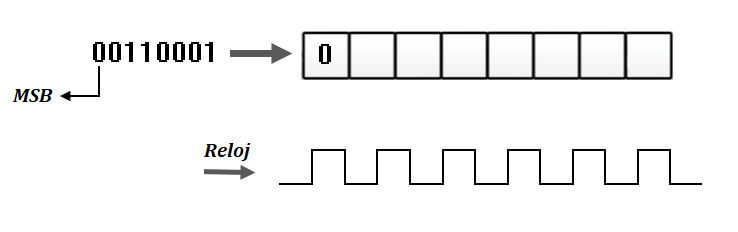
\includegraphics[scale=0.8]{MSB.png}
\centering
\caption{Entrada del MSB al integrado.}
\label{fig:MSB}
\end{figure}

En el próximo pulso del reloj el MSB, ya dentro del integrado, se correrá una posición a la derecha en el registro de desplazamiento, mientras que el número a la derecha del MSB, en la entrada, se posicionará en la primera posición del registro de desplazamiento.

\begin{figure}[h]
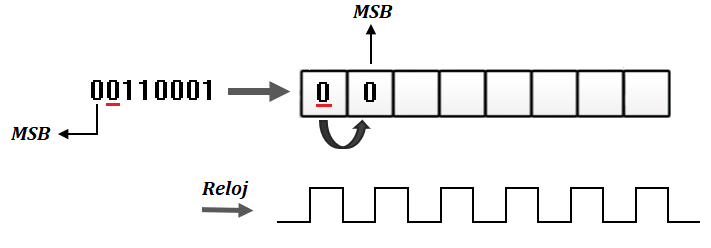
\includegraphics[scale=0.8]{MSB1.png}
\centering
\caption{Desplazamiento de los bits dentro del integrado.}
\label{fig:MSB1}
\end{figure}

Este proceso se repetirá hasta que se ingrese al registro de desplazamiento el último bit del número (Figura \ref{fig:registrolleno}).

\begin{figure}[h]
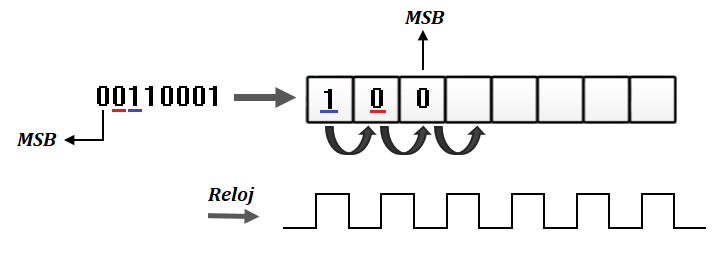
\includegraphics[scale=0.8]{BitsDespla.png}
\centering
\caption{Desplazamiento de los bits dentro del integrado.}
\label{fig:bitsdespla}
\end{figure}

\begin{figure}[h]
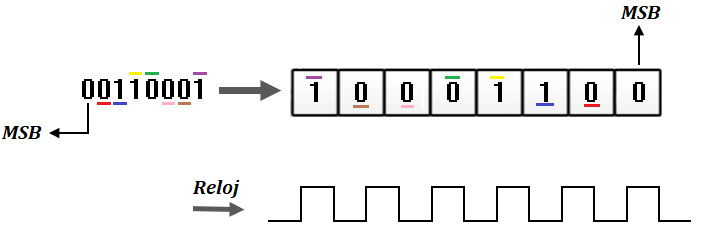
\includegraphics[scale=0.8]{registrolleno.png}
\centering
\caption{Registro de desplazamiento lleno. Se utilizaron colores encima o abajo de los bits para identificar fácilmente cuál es cuál en el registro de desplazamiento.}
\label{fig:registrolleno}
\end{figure}

Para que las salidas no vayan cambiando mientras que el registro de desplazamiento se llena, el integrado hace uso del registro de almacenamiento y el RCLK (Rejol del registro de almacenamiento).

\begin{figure}[h]
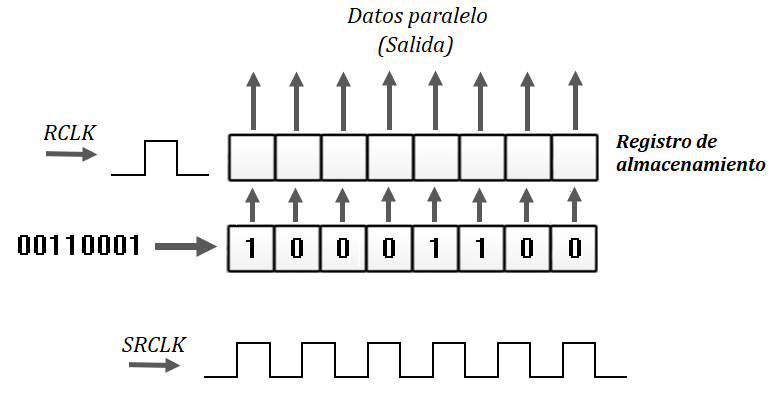
\includegraphics[scale=0.8]{regisalmacen.png}
\centering
\caption{Representación del registro de almacenamiento.}
\label{fig:registroalmacenamiento}
\end{figure}

















\newpage
\subsection{Aplicaciones.}\label{Aplicaciones}
\begin{itemize}
\item Network switches
\item Power infrastructure
\item LED displays
\item Servers
\end{itemize}


\section{Cibergrafía} \label{ciber}
(PONERLA CORRECTAMENTE)
https://www.electrogeekshop.com/como-funciona-el-74hc595-shift-register-y-su-interfaz-con-arduino/

\end{document}
